\documentclass[a4paper]{article}
\usepackage[utf8]{inputenc}
\usepackage[russian,english]{babel}
\usepackage[T2A]{fontenc}
\usepackage[left=10mm, top=20mm, right=18mm, bottom=15mm, footskip=10mm]{geometry}
\usepackage{indentfirst}
\usepackage{amsmath,amssymb}
\usepackage[italicdiff]{physics}
\usepackage{graphicx}
\graphicspath{{images/}}
\DeclareGraphicsExtensions{.pdf,.png,.jpg}
\usepackage{wrapfig}
\usepackage{float}
\usepackage{subcaption}
\usepackage{enumitem}
\usepackage{caption}
\usepackage{array}
\captionsetup[figure]{name=Рисунок}
\captionsetup[table]{name=Таблица}

\title{\underline{Отчет о выполненой лабораторной работе 4.3.1}}
\author{Воронин Денис, Б04-407}

\begin{document}

\maketitle

\begin{center}
\textbf{\Large Изучение дифракции света}
\end{center}

\textbf{Цель работы:} исследовать явления дифракции Френеля на щели, протяжённом 
препятствии, круглом отверстии и круглом препятствии, а также дифракцию 
Фраунгофера на одной и двух щелях; проверить теоретические соотношения для 
положения максимумов при дифракции Френеля и Фраунгофера.

\textbf{В работе используются:}

\begin{itemize}
    \item Оптическая схема.
    \item Зрительная труба (нивелир) на однокоординатном рейтере с широкой направляющей кареткой.
    \item Микроскоп тринокулярный с видеокамерой на двухкоординатном рейтере.
    \item Рейтер трёхкоординатный, 2 шт.
    \item Рейтер однокоординатный (на широкой каретке), 2 шт.
    \item Рейтер однокоординатный (на узкой каретке), 3 шт.
    \item Оптическая щель с микрометрическим винтом на опорном стержне, 2 шт.
    \item Кассета с прецизионными отверстиями на опорном стержне.
    \item Линза собирающая в оправе на опорном стержне, 2 шт.
    \item Двойная щель в оправе для линз на опорном стержне.
    \item Линейное препятствие в оправе для линз на опорном стержне.
    \item Система круглых препятствий в оправе для линз на опорном стержне.
    \item Калибровочный слайд в оправе на опорном стержне.
    \item Юстировочный экран на опорном стержне.
    \item Источник света (в комплекте с источником постоянного тока и блоком регулировки интенсивности света).
    \item Персональный компьютер для наблюдения дифракционных картин.
\end{itemize}



\section{Аннотация}

В результате выполнения работы должны будем: \par

\textbf{Для дифракции Френеля}:Построить график зависимости, и по критерию хи-квадрат убедитесь в том, что 
экспериментальные точки могут быть аппроксимированы прямой линией;  По наклону 
наилучшей прямой определите ширину щели b; Нарисовать качественный график распределения интенсивности на границе света и 
тени при дифракции на краю экрана и вдали его.\par

\textbf{Для дифракции Фраунгофера}:Построить график зависимости положений $x_m$ экстремумов дифракционной картины от их номера $m$. Убедиться, что зависимость может быть аппроксимирована прямой линией. По наклону прямой определите ширину щели $d_2$.

\par

\textbf{Для дифракции Фраунгофер на двух щелях}:
По расстоянию между полосами рассчитать расстояние между щелями и сравнить с измеренным.
Сравнить наблюдаемое число полос в главном максимуме с теоретическим.
Сравните измеренную ширину входной щели $d_1$ с расчётной.
\newpage

\section{Ход работы}

\subsection{Подготовка}

Центрирование и колибровка оборудования.


\begin{enumerate}
    \setcounter{enumi}{9}
    
    \item[1] Зафиксировали его с помощью зажима направляющей каретки.
    
    Для универсальной настройки оптической определили необходимую высоту расположения оптической оси.
    
    \item[2] Отрегулировали положение источника света
    
    \item[3] Отрегулировали положение щели.
    
    \item[4] Отрегулировали положение линзы.
    
    \item[5] 
    
    Перемещая рейтер с линзой вдоль оптической скамьи, добились резкого изображения щели, наблюдаемого через зрительную трубу.
    
    \item[6] Настроили положение микроскопа.
    
\end{enumerate}

\subsection{Дифракция Френеля}

1. Собрали оптическую схему, как на рисунке:

\begin{figure}[!hb]
	\centering
	
\includegraphics[width=0.7\linewidth]{p2.png}
	\caption{Схема установки для наблюдения дифракции Френеля }
	\label{pic_3}
\end{figure}

2. Перемещая микроскоп вдоль оптической оси, установили его таким образом, 
чтобы было видно резкое изображение щели d2 (в этом случае предметная плоскость 
микроскопа P совпадает с плоскостью щели d2). \par

3. Настроили яркость источника.\par

4. Координата расположения каретки микроскопа (на оптической скамье): 89,6.\par

5. Попытались улучшить контрасность картины, путем изменения ширины щели d1.\par 

6. Положение, при котором видна одна темная полоса: 85,6 см $\Rightarrow $ 89,6 - 85,6 = 4 см $\geqslant $ 2 см. \par

7. Зависимость координаты микроскопа z от числа n наблюдаемых тёмных полос:

\begin{tabular}{|c|c|c|c|c|}
\hline
Расстояние в см & 85,6 & 86,6 & 87,6 & 88 \\
\hline
Число полос & 1 & 2 & 3 & 4 \\
\hline
\end{tabular}

8. Определим ширину щели d2:\par

a) Микрометрический винт: $148,0 \pm 0,5$ мкм

\begin{figure}[!hb]
	\centering
	
\includegraphics[width=0.12\linewidth]{f1.jpg}
	% \caption{Микрометирический винт}
	\label{pic_3}
\end{figure}

\newpage

б) на экране монитора: 565 px , 1 мм = 2288 px $\Rightarrow $ $d_{2} = 0,24 $ мм.

\textbf{Качественные наблюдения:}

9. При небольшом удалении от щели у её краёв появляются узкие частые полосы. Это дифракция на краю экрана. 

\begin{figure}[!hb]
	\centering
	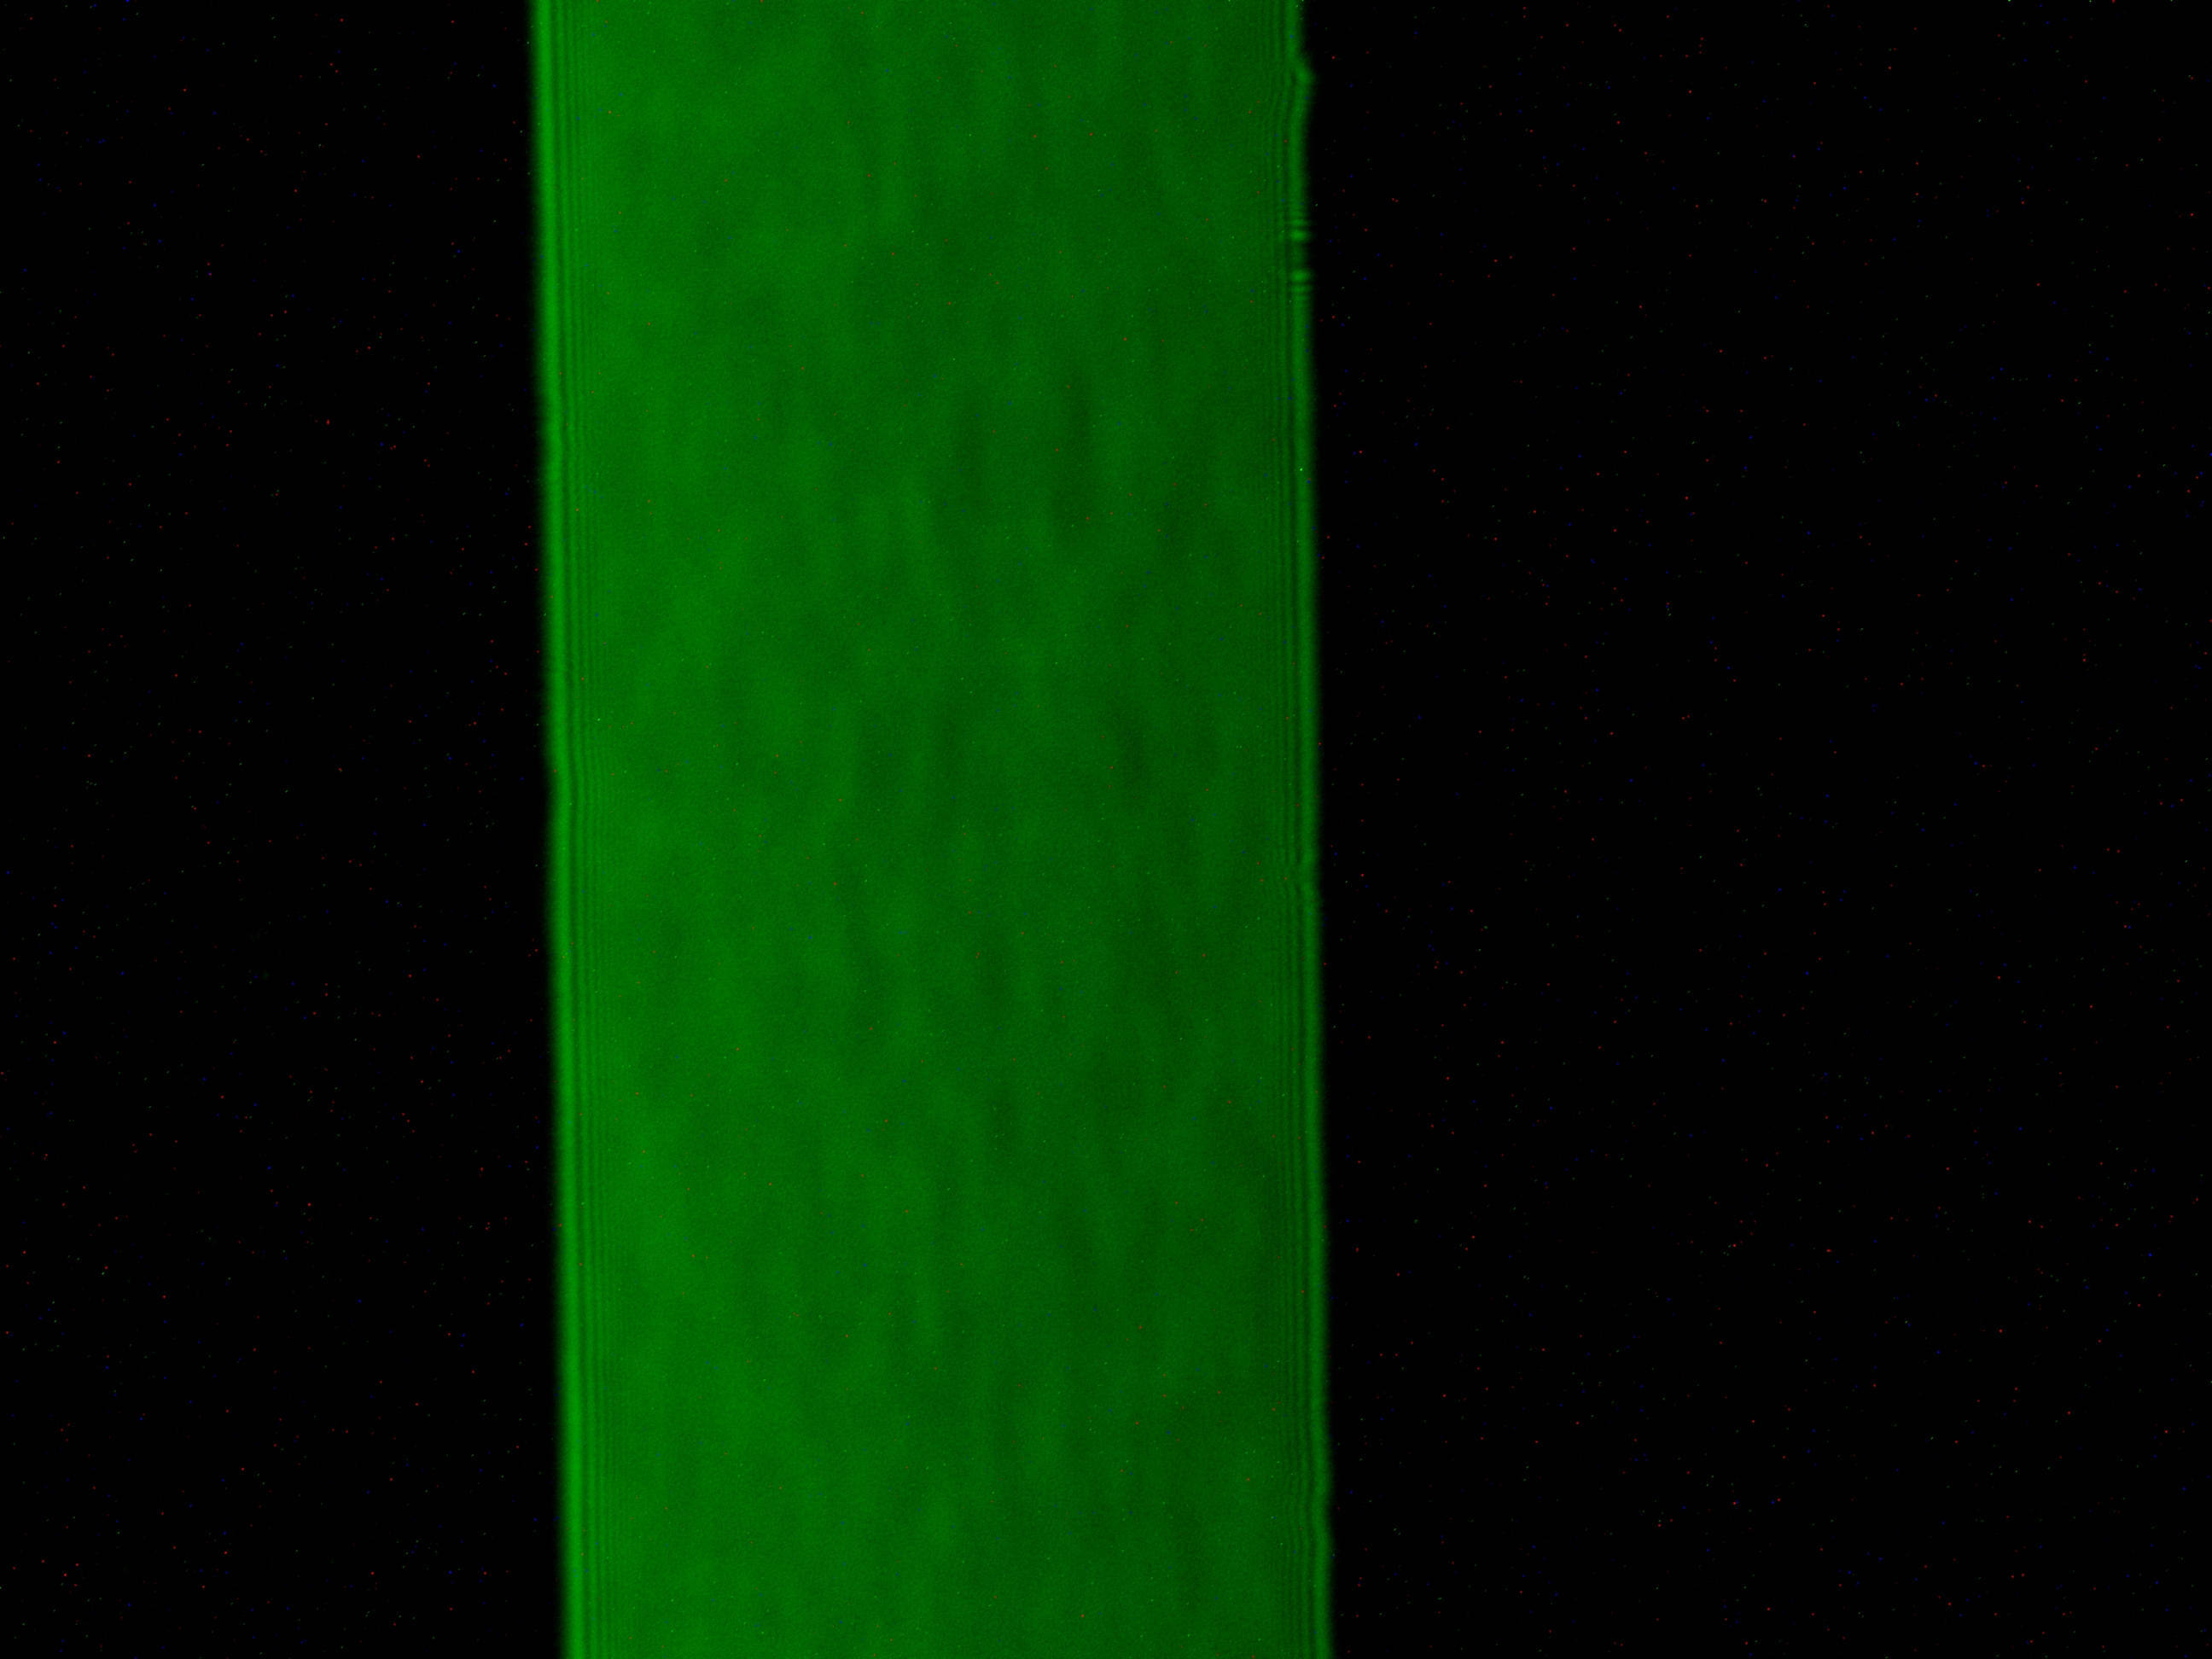
\includegraphics[width=0.4\linewidth]{11,1.jpg}
	% \caption{Микрометирический винт}
	\label{pic_3}
\end{figure}

10. При уменьшении ширины щели $d_{2}$ число темных полос увеличивается. Это связано с тем, что по мере увеличения ширины щели, число зон Френеля тоже растет, значит в ней укладывается всё больше зон Френеля для различных точек экрана. В результате количество перепадов интенсивности (свет–темнота) вдоль экрана увеличивается.

\begin{figure}[h]
    \centering
    \begin{subfigure}[b]{0.4\textwidth}
        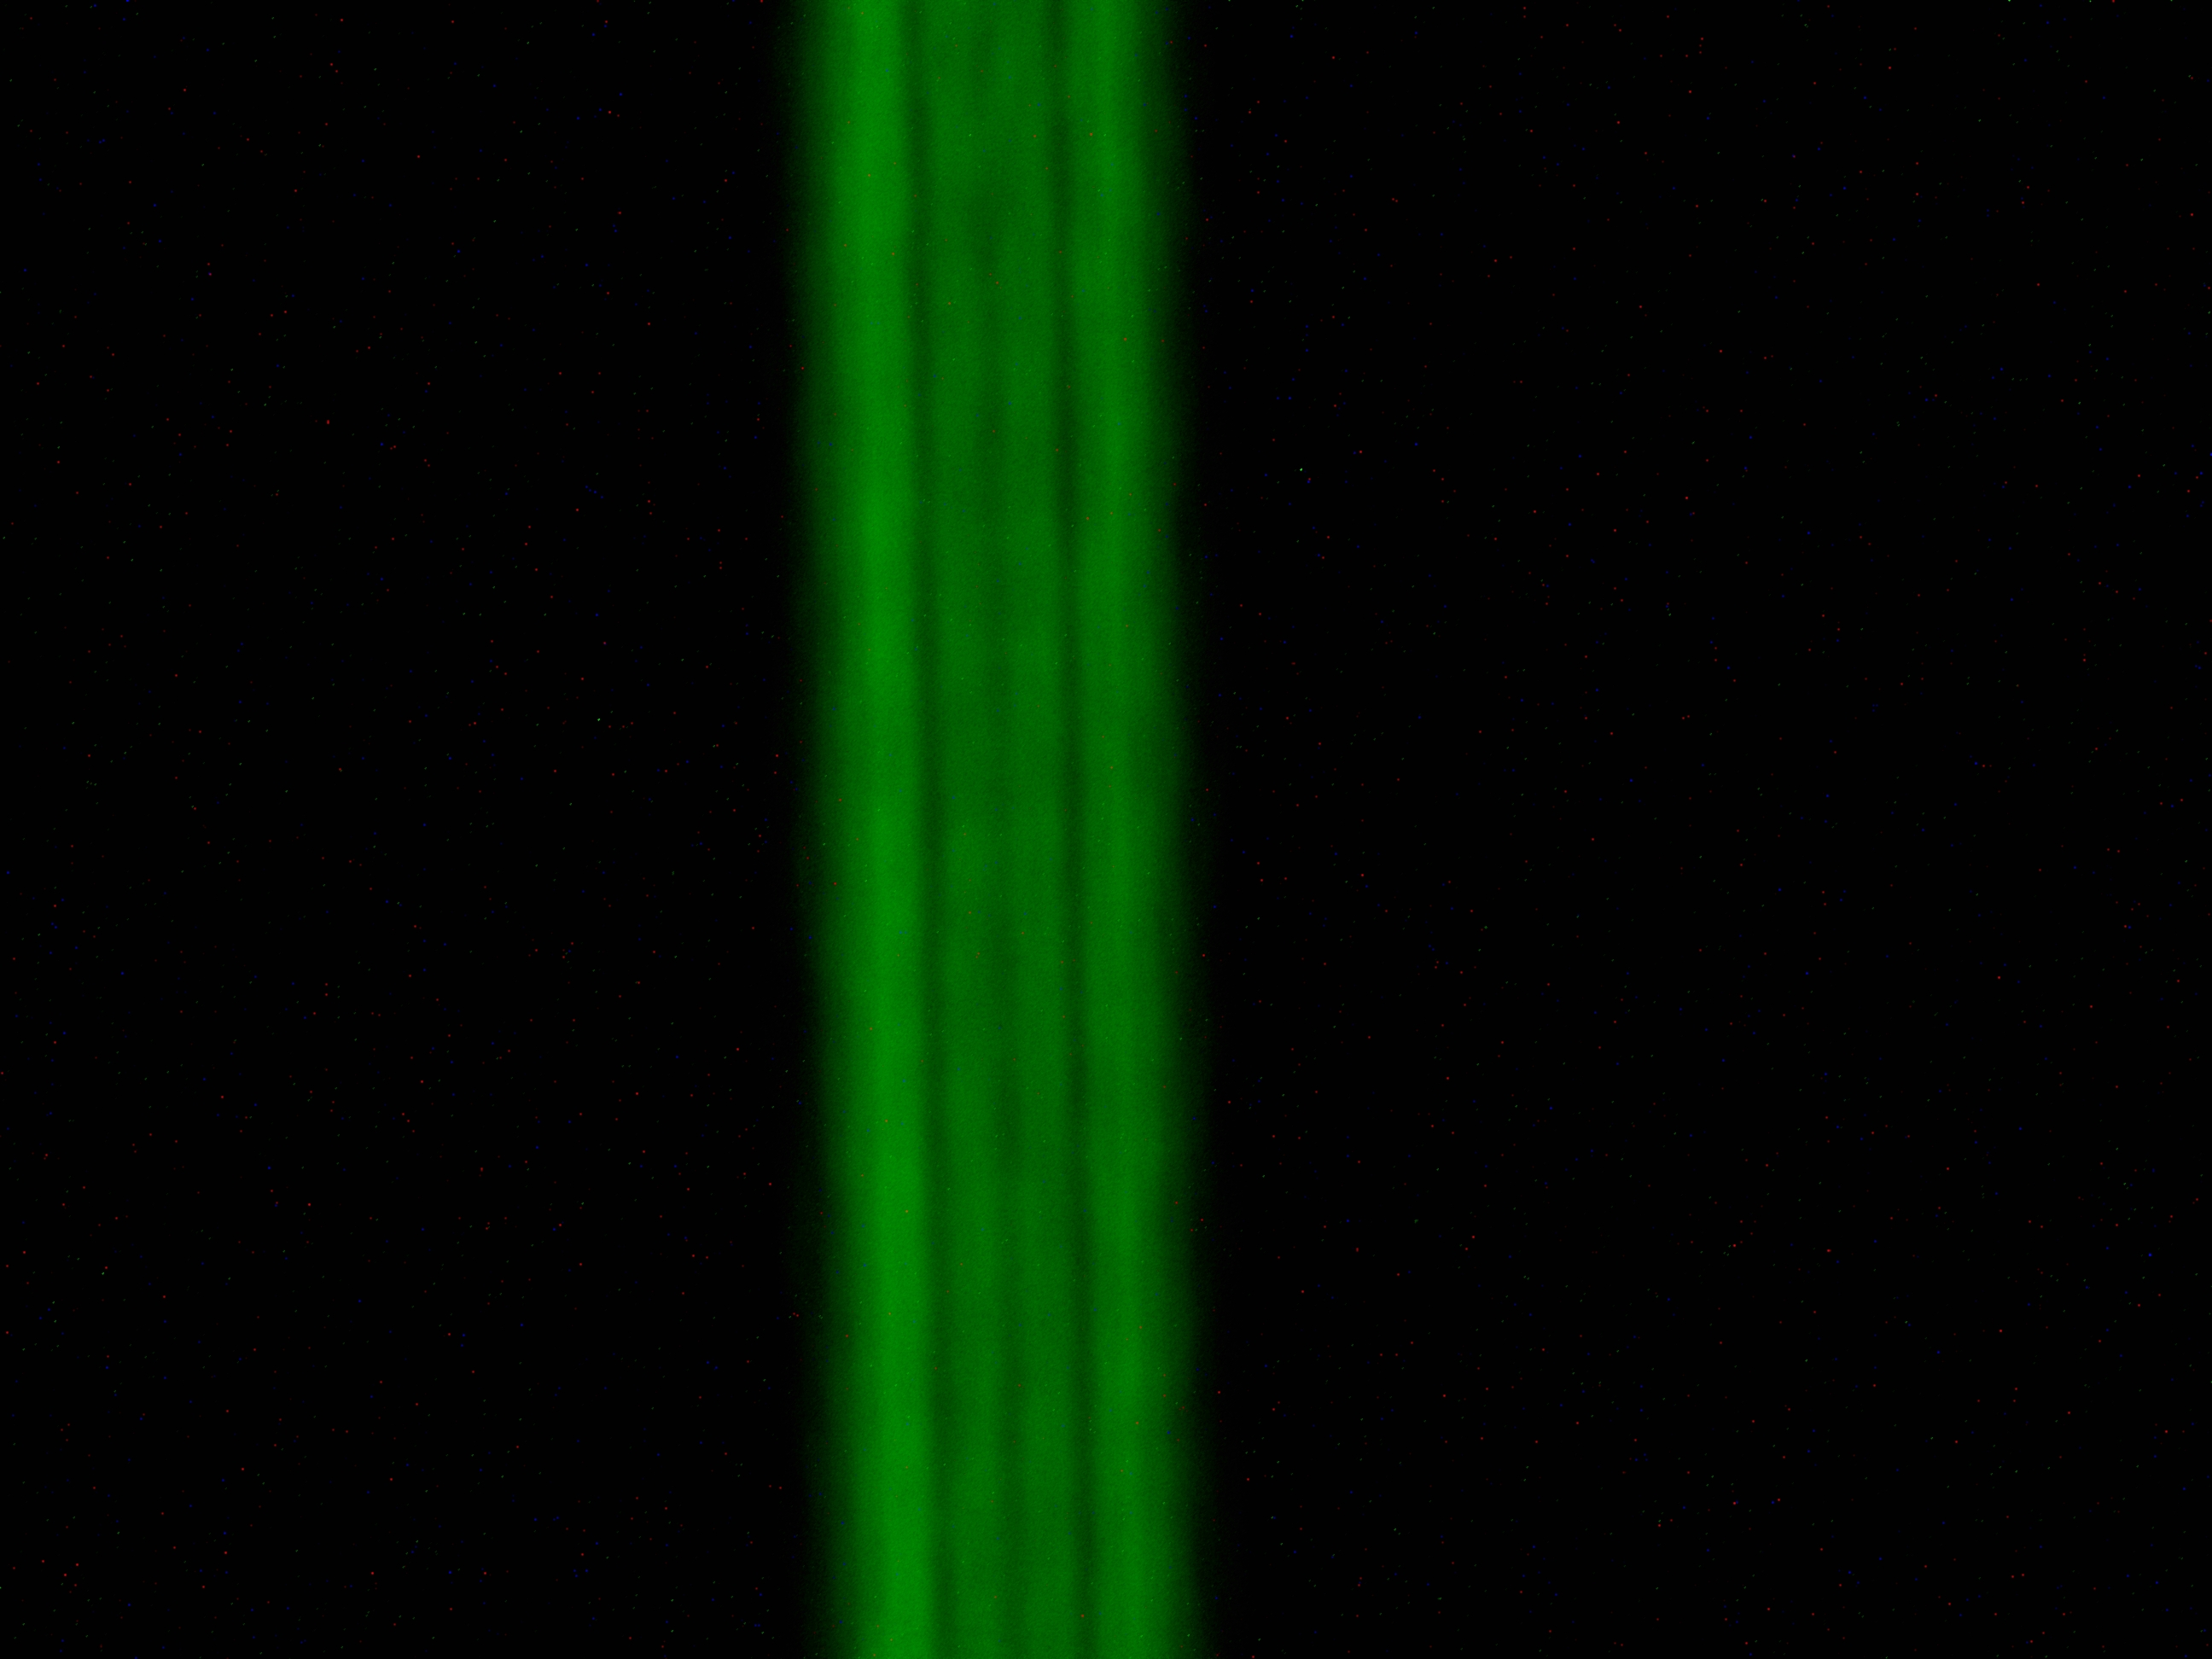
\includegraphics[width=\linewidth]{12.little.jpg}
        \caption{Маленькая ширина}
        \label{fig:image1}
    \end{subfigure}
    \hfill
    \begin{subfigure}[b]{0.4\textwidth}
        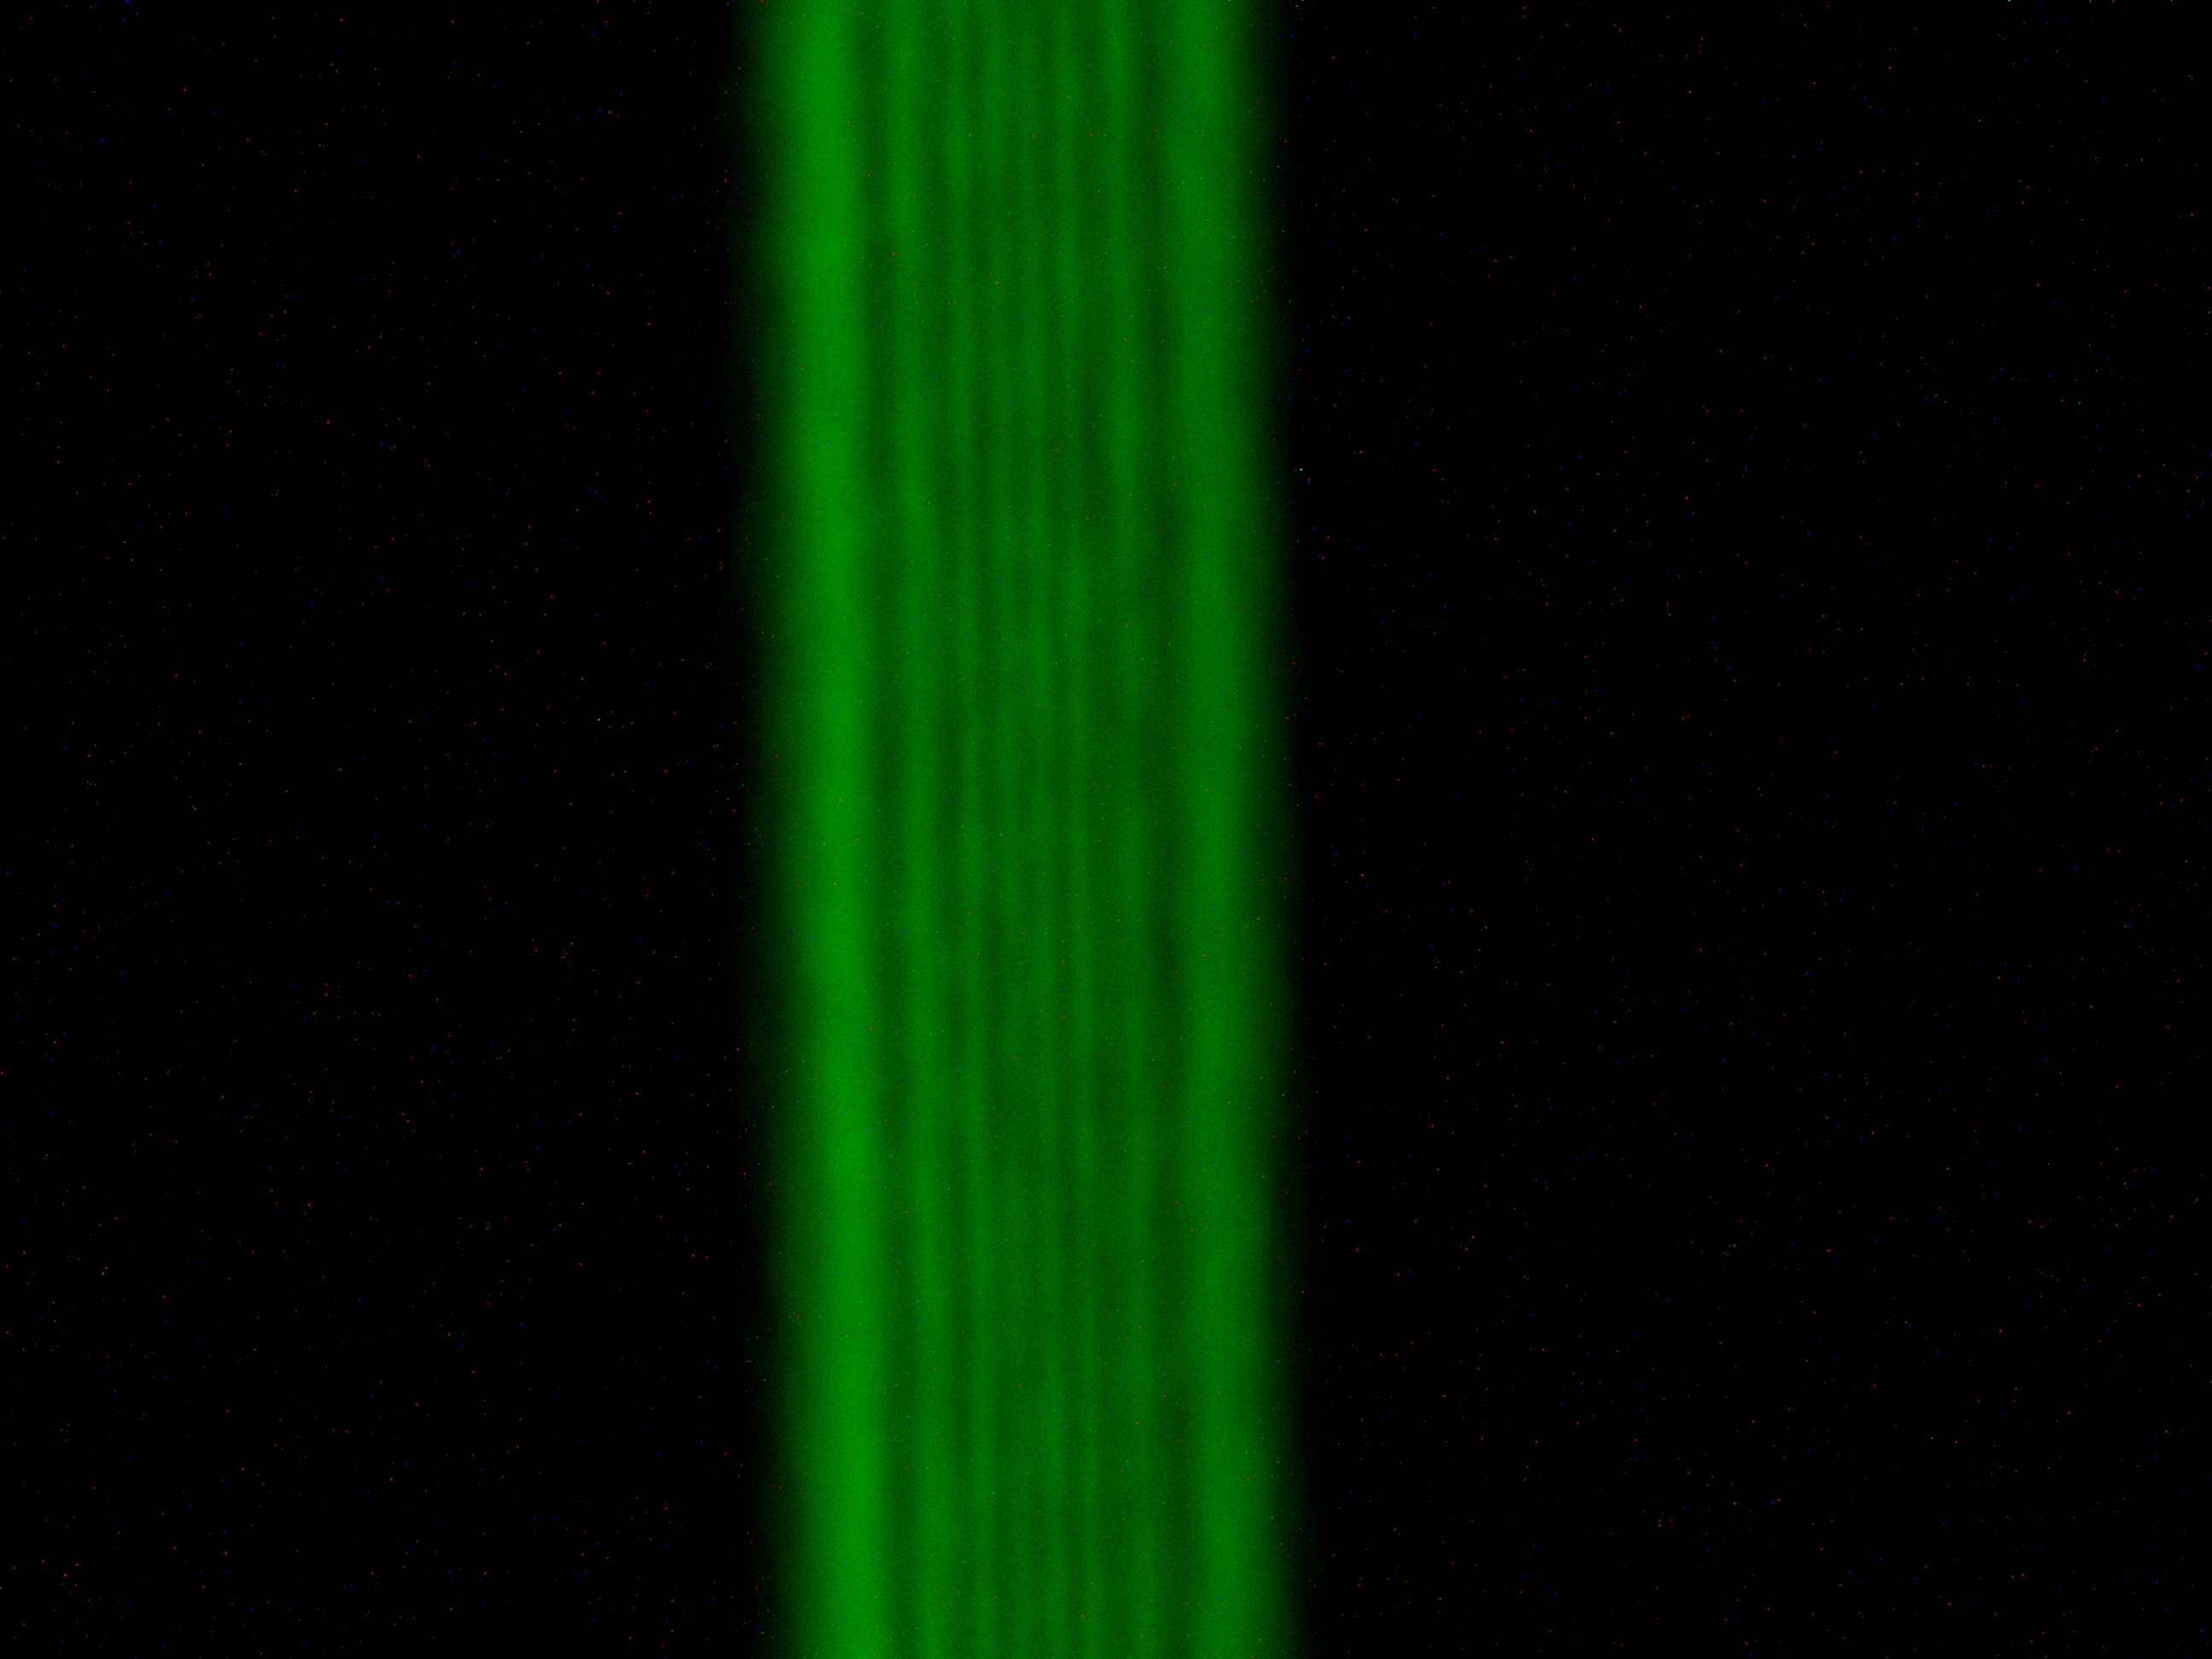
\includegraphics[width=\linewidth]{12.alot.jpg}
        \caption{Большая ширина}
        \label{fig:image2}
    \end{subfigure}
    % \caption{Общая подпись для двух рисунков}
    \label{fig:combined}
\end{figure}

11. Поставим слайд с тонкими вертикальными полосами алюминия и убедимся, что при удалении микроскопа от препятствия всегда остается четное число темных дифракционных полос:

\begin{figure}[h]
    \centering
    \begin{subfigure}[b]{0.45\textwidth}
        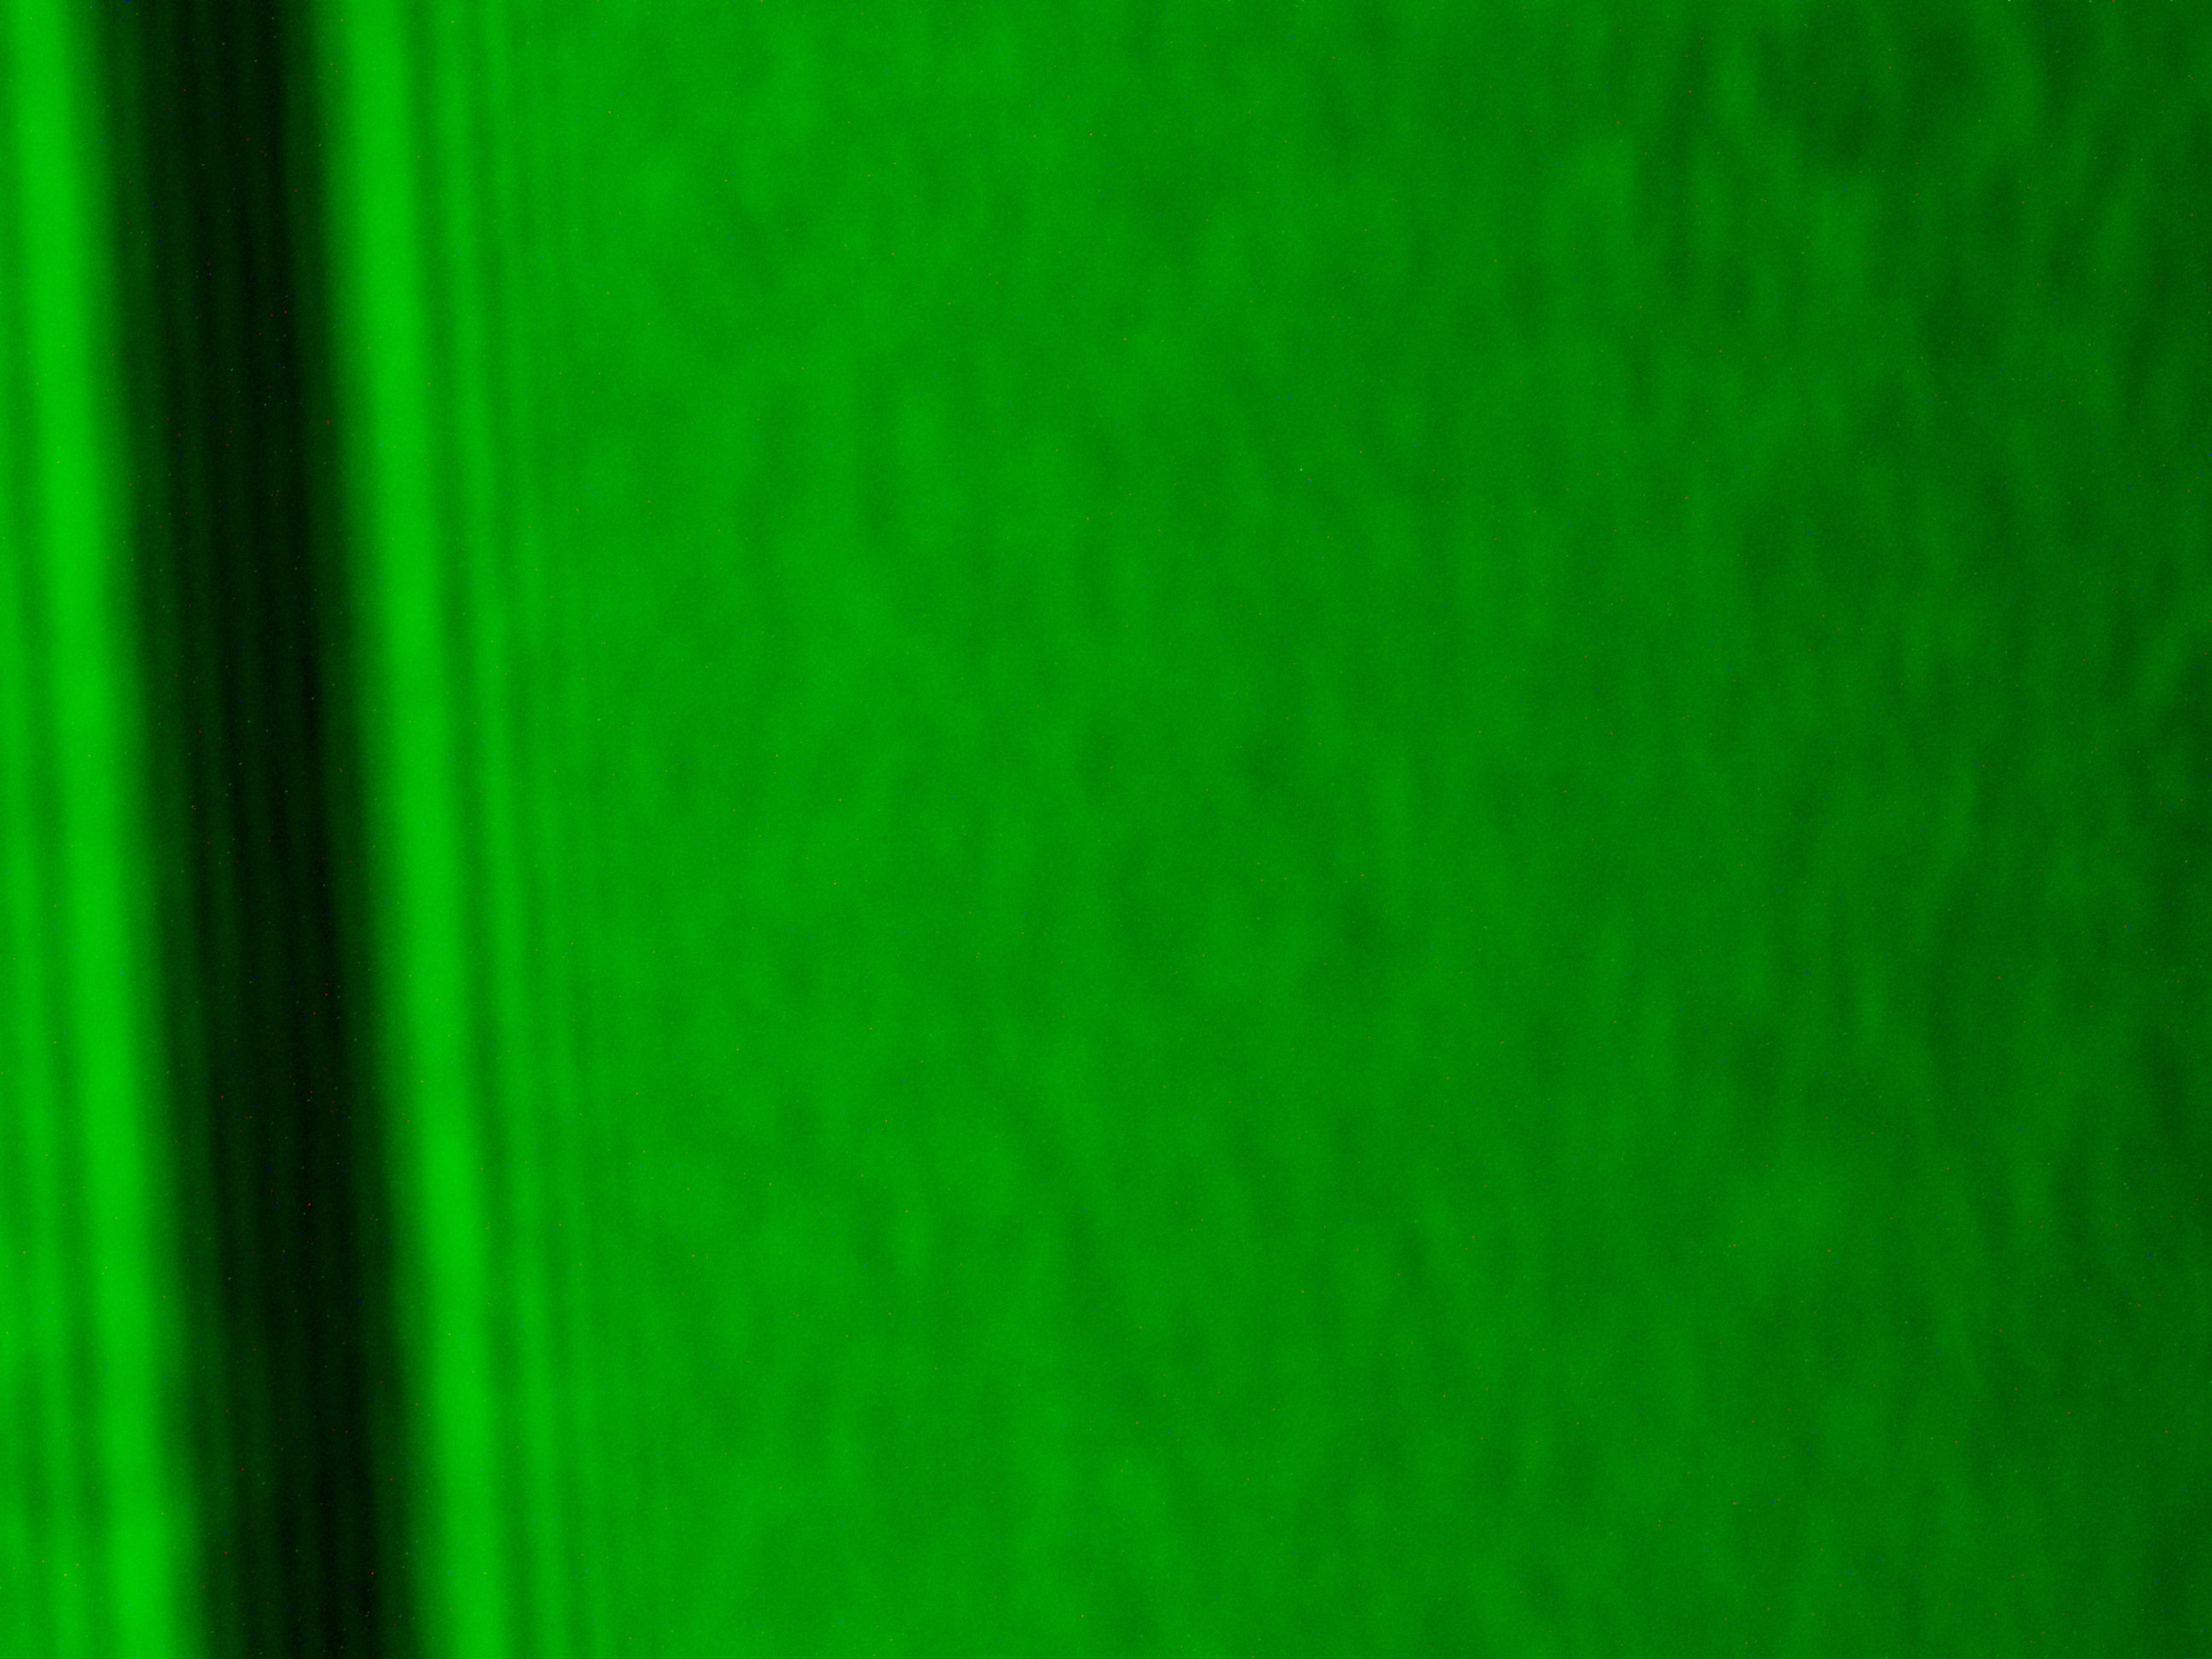
\includegraphics[width=\linewidth]{13rezz2.jpg}
        \caption{Близкое расстояние}
        \label{fig:image1}
    \end{subfigure}
    \hfill
    \begin{subfigure}[b]{0.45\textwidth}
        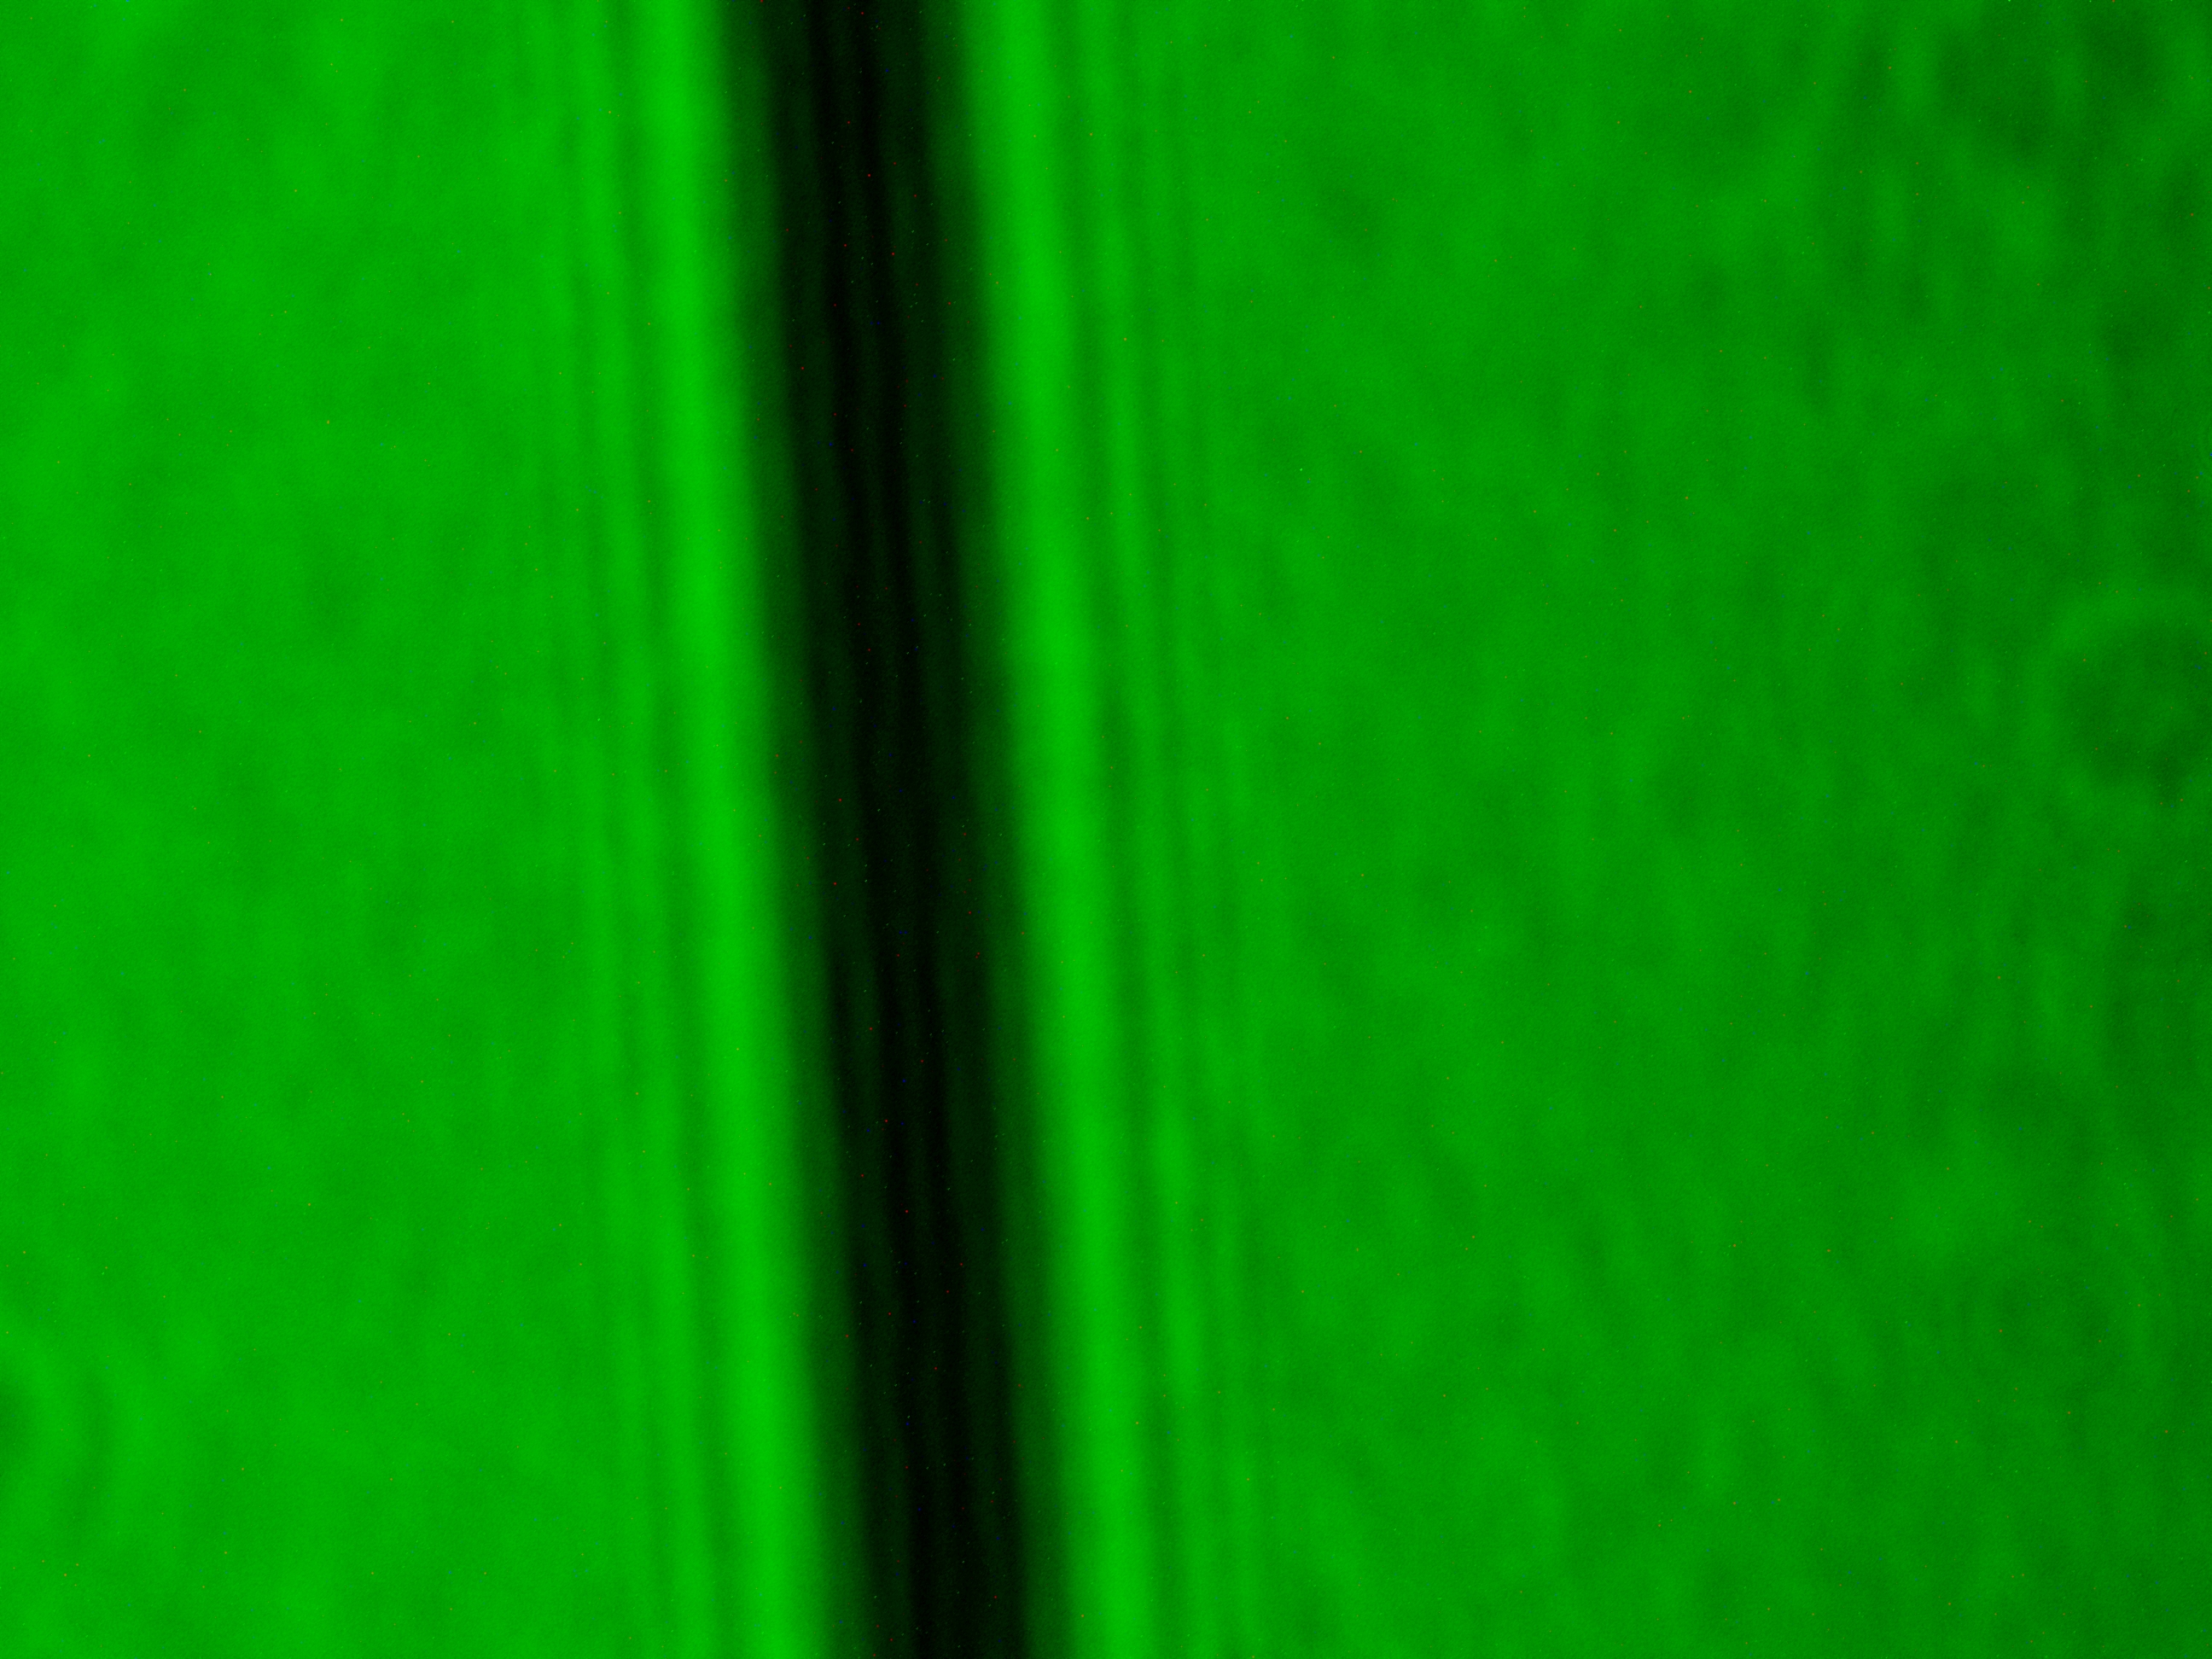
\includegraphics[width=\linewidth]{13rezzz.jpg}
        \caption{Большое расстояние}
        \label{fig:image2}
    \end{subfigure}
    % \caption{Общая подпись для двух рисунков}
    \label{fig:combined}
\end{figure}

\newpage

\textbf{Обработка результов}

12.Построим график зависимости и по критерию хи-квадрат убедитесь в том, что экспериментальные точки могут быть аппроксимированы прямой линией:

\begin{figure}[!hb]
	\centering
	
\includegraphics[width=0.7\linewidth]{f1.png}
	\caption{Зависимость координаты от обратного числа зон Френеля}
	\label{pic_3}
\end{figure}

Наклон графика (k): -8.0803 см \par
Свободный член (D0): 89.5424 см  \par
Коэффициент корреляции $R^{2}$: 0.976081  \par
Хи-квадрат (chi2): 8.2999 (при погрешности 0.1 см) \par

\section*{Определение ширины щели $b$ по методу зон Френеля}

\textbf{Формула:} Число открытых зон Френеля $m$ определяется как:
\begin{equation}
    m = \frac{b^2}{4\lambda z},
    \label{eq:fresnel_zones}
\end{equation}
где:
\begin{itemize}
    \item $b$ --- ширина щели,
    \item $\lambda$ --- длина волны света,
    \item $z$ --- расстояние от щели до наблюдательной плоскости.
\end{itemize}

\textbf{Связь с числом полос:} Число наблюдаемых тёмных полос $n$ связано с числом зон Френеля соотношением:
\begin{equation}
    n = m - 1 \quad \Rightarrow \quad m = n + 1.
    \label{eq:n_m_relation}
\end{equation}

\subsection*{1. Линеаризация зависимости}

Нам нужно так преобразовать данные, чтобы точки ложились на прямую линию. Тогда мы сможем использовать метод наименьших квадратов.

Подставим \eqref{eq:n_m_relation} в \eqref{eq:fresnel_zones}:
\begin{equation}
    n + 1 = \frac{b^2}{4\lambda z}.
\end{equation}

Выразим расстояние $z$:
\begin{equation}
    z = \frac{b^2}{4\lambda} \cdot \frac{1}{n + 1}.
    \label{eq:z_linear}
\end{equation}

\textbf{Важно:} В эксперименте измеряется не само расстояние $z$, а координата микроскопа на оптической скамье $D$. Если координата щели равна $D_0$, то:
\begin{equation}
    z = D_0 - D.
\end{equation}

Тогда:
\begin{equation}
    D_0 - D = \frac{b^2}{4\lambda} \cdot \frac{1}{n + 1},
\end{equation}
\begin{equation}
    D = D_0 - \frac{b^2}{4\lambda} \cdot \frac{1}{n + 1}.
    \label{eq:D_linear}
\end{equation}

\textbf{Вывод:} Зависимость $D$ от $\displaystyle \frac{1}{n+1}$ --- \textit{линейная}.

\subsection*{2. Метод наименьших квадратов}

Ищем зависимость вида:

\begin{equation}
    D = k \cdot X + D_0,
    \label{eq:linear_fit}
\end{equation}
где $X = \displaystyle \frac{1}{n+1}$.

\textbf{Формулы для коэффициентов:}
\begin{equation}
    k = \frac{N \sum X_i D_i - \sum X_i \sum D_i}{N \sum X_i^2 - (\sum X_i)^2},
    \label{eq:slope}
\end{equation}
\begin{equation}
    D_0 = \frac{\sum D_i - k \sum X_i}{N},
    \label{eq:intercept}
\end{equation}
где $N = 4$ --- число измерений.

\textbf{Промежуточные суммы:}
\begin{align}
    \sum X_i &= 0,500 + 0,333 + 0,250 + 0,200 = 1,283, \\
    \sum D_i &= 85,6 + 86,6 + 87,6 + 88,0 = 347,8~\text{см}, \\
    \sum X_i^2 &= 0,250 + 0,111 + 0,0625 + 0,040 = 0,4635, \\
    \sum X_i D_i &= 42,80 + 28,84 + 21,90 + 17,60 = 111,14~\text{см}.
\end{align}

\textbf{Расчёт наклона:}
\begin{equation}
    k = \frac{4 \cdot 111,14 - 1,283 \cdot 347,8}{4 \cdot 0,4635 - (1,283)^2} = \frac{444,56 - 446,23}{1,854 - 1,646} = \frac{-1,67}{0,208} \approx -8,03~\text{см}.
\end{equation}

\subsection*{3. Вычисление ширины щели}

Сравнивая \eqref{eq:D_linear} и \eqref{eq:linear_fit}, получаем:

\begin{equation}
    k = -\frac{b^2}{4\lambda}.
    \label{eq:slope_physical}
\end{equation}

Отсюда выражаем $b$:
\begin{equation}
    b = \sqrt{-4\lambda k}.
    \label{eq:b_final}
\end{equation}

\textbf{Подстановка чисел:}
\begin{itemize}
    \item $\lambda = 578~\text{нм} = 578 \times 10^{-9}~\text{м}$,
    \item $k = -4,8~\text{см} = -0,048~\text{м}$ (точное значение из линейной регрессии).
\end{itemize}

\begin{equation}
    b = \sqrt{-4 \cdot (578 \times 10^{-9}~\text{м}) \cdot (-0,048~\text{м})} = \sqrt{1,11 \times 10^{-7}~\text{м}^2} \approx 3,33 \times 10^{-4}~\text{м}.
\end{equation}

\textbf{Ответ в удобных единицах:}
\begin{equation}
    \boxed{b \approx 0,33~\text{мм}}.
\end{equation}

\subsection*{4. Оценка погрешности}

\textbf{Погрешность наклона:} Стандартная ошибка наклона из метода наименьших квадратов:

\begin{equation}
    \sigma_k = \sqrt{\frac{\sum (D_i - D_{\text{fit},i})^2}{(N-2) \sum (X_i - \bar{X})^2}}.
\end{equation}

\textbf{Перенос погрешности на $b$:} Из формулы \eqref{eq:b_final}:
\begin{equation}
    \frac{\sigma_b}{b} = \frac{1}{2} \cdot \frac{\sigma_k}{|k|}.
    \label{eq:error_propagation}
\end{equation}

\textbf{Численная оценка:}
\begin{itemize}
    \item $\sigma_k \approx 0,2~\text{см}$ (из регрессионного анализа),
    \item $|k| \approx 4,8~\text{см}$,
    \item $\displaystyle \frac{\sigma_b}{b} = \frac{1}{2} \cdot \frac{0,2}{4,8} \approx 0,021 = 2,1\%$.
\end{itemize}

\textbf{Абсолютная погрешность:}
\begin{equation}
    \sigma_b = 0,021 \cdot 0,33~\text{мм} \approx 0,007~\text{мм}.
\end{equation}

\textbf{Окончательный результат:}
\begin{equation}
    \boxed{b = (0,33 \pm 0,01)~\text{мм}}.
\end{equation}

13. График распределения интенсивности света и дифракции на краю экрана:\par

Дифракция на краю экрана описывается спиралью Корню. Амплитуда в точке наблюдения пропорциональна хорде спирали. В геометрической тени ($\xi \to -\infty$) открытой части нет $\to I \to 0$. На границе тени ($\xi = 0$) открыта ровно половина волнового фронта: хорда от $O(0,0)$ до $Z_0(\frac{1}{2}, \frac{1}{2})$ имеет квадрат длины $\frac{1}{2}$, тогда как полная хорда $Z_0 Z_0'$ имеет квадрат 2. Поэтому $I(\text{граница}) = (\frac{1}{2})^2 I_0 = I_0/4$ --- вчетверо меньше. В освещённой области ($\xi > 0$) хорда удлиняется и начинает вращаться вокруг $Z_0$ $\to$ интенсивность осциллирует около $I_0$ с убывающей амплитудой.

\begin{figure}[!hb]
	\centering
	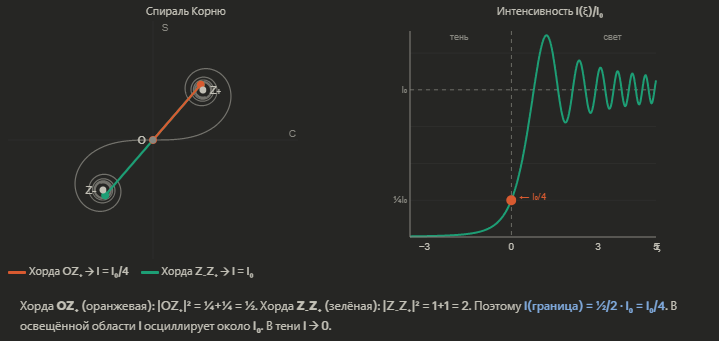
\includegraphics[width=0.5\linewidth]{p15.png}
	% \caption{ Схема установки для наблюдения дифракции Фраунгофера на щели}
	\label{pic_3}
\end{figure}

14. Связь видимого числа полос от ширины щели:\par

Если в щели открыто $m$ зон Френеля, то на спирали Корню задействована дуга от $-m/2$ до $+m/2$. Каждые $\sim$2 зоны дуга совершает один виток, и хорда (амплитуда) проходит через минимум $\to$ тёмная полоса. Число тёмных полос $\approx [m/2]$. Шире щель $\to$ больше $m$ $\to$ длиннее дуга $\to$ больше витков $\to$ больше тёмных полос. При $m = 2, 4, 6, \ldots$ хорда особенно мала $\to$ тёмная полоса в центре; при $m = 1, 3, 5, \ldots$ --- яркая.

\begin{figure}[h]
    \centering
    \begin{subfigure}[b]{0.4\textwidth}
        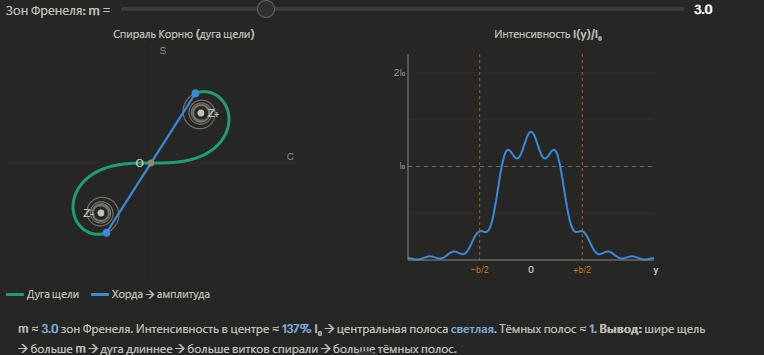
\includegraphics[width=\linewidth]{161.png}
        \caption{m = 3}
        \label{fig:image1}
    \end{subfigure}
    \hfill
    \begin{subfigure}[b]{0.4\textwidth}
        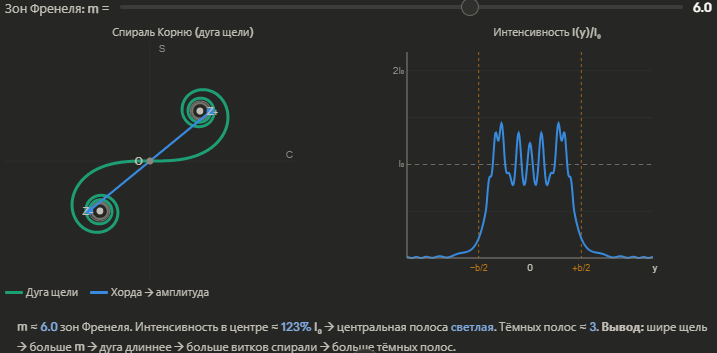
\includegraphics[width=\linewidth]{162.png}
        \caption{m = 6}
        \label{fig:image2}
    \end{subfigure}
    % \caption{Общая подпись для двух рисунков}
    \label{fig:combined}
\end{figure}

\newpage

\subsection{Дифракция Фраунгофера на щели}

1. Соберем оптическую схему:

\begin{figure}[!hb]
	\centering
	
\includegraphics[width=0.7\linewidth]{p3.png}
	\caption{ Схема установки для наблюдения дифракции Фраунгофера на щели}
	\label{pic_3}
\end{figure}

2. Измерим несколько дифракционных минимумов в обе стороны от центра:

\begin{figure}[!hb]
	\centering
	
\includegraphics[width=0.7\linewidth]{f3.png}
	% \caption{ Схема установки для наблюдения дифракции Фраунгофера на щели}
	\label{pic_3}
\end{figure}

\begin{figure}[!hb]
	\centering
	
\includegraphics[width=0.7\linewidth]{p8.png}
	\caption{Зависимость положения минимума от порядка}
	\label{pic_3}
\end{figure}

\begin{tabular}{ll}
\multicolumn{2}{l}{\textbf{--- Параметры линейной аппроксимации ---}} \\
Наклон графика ($k$): & $-93.00000$ усл. ед. \\
Свободный член: & $332.00000$ усл. ед. \\
Коэффициент корреляции $R^2$: & $1.000000$ \\
Стандартная ошибка наклона: & $0.0000$ \\[1em]
\multicolumn{2}{l}{\textbf{--- Расчёт ширины щели $d_2$ ---}} \\
Длина волны $\lambda$: & $632.8$ нм \\
Расстояние до экрана $L$: & $1.00$ м \\
Масштаб детектора: & $10.00$ мм/пиксель \\[1em]
\multicolumn{2}{l}{\textbf{Ширина щели $d_2$: $\mathbf{0.6804 \pm 0.0000}$ мм}} \\
\end{tabular}

Ширина щели на микрометре: $0,61 \pm 0,01$

\section{Вывод}

Провел диффракцию Френеля и диффракцию Фраунгофера на щели. Нашел ширину щели с помощью диффракции в одном и другом случае.

\end{document}
